\documentclass[doc,floatsintext]{apa6}
\usepackage[american]{babel}
\usepackage{csquotes}
\usepackage{apacite}
\usepackage[T1]{fontenc}
\usepackage{lmodern}
\usepackage[utf8]{inputenc}
\usepackage{amssymb}
\usepackage{amsfonts}
\usepackage{amsmath}
\usepackage{graphicx}
\usepackage{float}
\usepackage{caption}
\usepackage{subcaption}
\usepackage{enumitem}
\usepackage[section]{placeins}
\usepackage[textsize=tiny]{todonotes}
\bibliographystyle{apacite}
\setlength{\marginparwidth}{2cm}

% ---------- paper specific ---------
\newcommand{\mat}[1]{\mathbf{#1}}
\newcommand{\vect}[1]{\mathbf{#1}}

% ---------- watermark -----------
\usepackage[firstpage]{draftwatermark}
\SetWatermarkAngle{0}
\SetWatermarkFontSize{0.25cm}
\SetWatermarkVerCenter{0.75cm}
\SetWatermarkLightness{0.5}
\SetWatermarkHorCenter{14cm}
\SetWatermarkText{\shortstack[l]{
Navarro, D. J. (2003). Regarding the complexity of additive clustering models: \\
Comment on Lee (2001). Journal of Mathematical Psychology, 47, 241-243 \\
http://dx.doi.org/10.1016/S0022-2496(02)00026-3
}}
\SetWatermarkScale{1}
% -------------------------------

\title{Regarding the complexity of additive clustering models: Comment on Lee (2001)}
\author{\normalsize Danielle J. Navarro}
\affiliation{Department of Psychology \\ University of Adelaide}
\date{}
\shorttitle{}

\abstract{The additive clustering approach to modeling pairwise similarity of entities is a powerful tool for deriving featural stimulus representations. In a recent paper, \citeA{lee01b} proposes a statistically principled measure for choosing between clustering models that accounts for model complexity as well as data fit. Importantly, complexity is understood to be a property, not merely of the number of clusters, but also their size and pattern of overlap. However, some caution is required when interpreting the measure, with regard to the applicability of the Hadamard inequality to the complexity matrix.}

\begin{document}
\maketitle

\vspace{12pt}
Additive clustering \cite{sheara79} represents a simple and effective method for modeling the similarity between a set of $n$ stimuli. Clustering algorithms that fit the additive clustering model input a matrix of pairwise similarities $\mat{S}=[s_{ij}]$ and derive a stimulus representation in the form of a set of $m$ saliency-weighted clusters (sometimes interpreted as features). Formally, the model consists of an $n \times m$ feature matrix $\mat{F}=[f_{ik}]$ where $f_{ik}$ is 1 if the $i$-th stimulus possesses the $k$-th feature, and 0 if it does not, as well as a vector of nonnegative saliency weights $\vect{w}=[w_{k}]$. An additive clustering representation estimates the similarity between two stimuli by the sum of the weights of shared features: that is to say, $\hat{s}_{ij}=\sum_{k} w_{k}f_{ik}f_{jk}$. It is common practice to include a nonnegative ``additive constant'', added to all similarity estimates, which can be regarded as a mandatory extra cluster encompassing all stimuli.

An important theoretical issue in additive clustering regards how to choose between featural representations. In a recent paper, \citeA{lee01b} proposes a measure that approximates the Bayesian posterior probability by employing an established variant on Laplace's method (see \citeNP{kasraf95}). This measure provides a trade off between goodness-of-fit and model complexity, and importantly, the measure of complexity is sensitive to the interaction between clusters, as well as to their number. The key component of this measure is the determinant of the \emph{complexity matrix} $\mat{G}=[g_{xy}]$, the $m \times m$ matrix such that $g_{xy}=g_{yx}=\sum_{i<j} f_{ix}f_{jx}f_{iy}f_{jy}$. In other words, the $xy$-th element of $\mat{G}$ counts the number of pairs of stimuli that share the $x$-th feature and the $y$-th feature. Main diagonal elements of $\mat{G}$ are given by the number of pairs of stimuli that share a single feature: that is, $g_{xx}$ reduces to $\sum_{i<j} f_{ix}f_{jx}$. Correspondingly, a row (or column) in $\mat{G}$ reflects both the size of a cluster and the extent of its overlap with other clusters. This complexity matrix has broad applicability, also appearing in expressions for the Stochastic Complexity (Rissanen, \citeyearNP{ris96}; see also Lee, \citeyearNP{leesub3}) and the related Geometric Complexity  \cite{myubalpit00} for additive clustering representations.

Lee demonstrates that for non-degenerate feature structures, $\mat{G}$ is positive definite, and applies Hadamard's inequality \cite[pp. 129-130]{bel70}, which states that the determinant of $\mat{G}$ is less than or equal to the product of its main diagonal,

\begin{displaymath}
\label{eq:hadamard}
|\mat{G}| \leq \prod_{x} \sum_{i<j} f_{ix} f_{jx}
\end{displaymath}

\noindent
with equality occurring when all off-diagonal elements are zero. From this observation Lee argues that, for a fixed number of clusters, the most complex representation is a partition, in which every stimulus belongs to precisely one cluster, since these models have diagonal complexity matrices. However, it should be observed that although all partitions have diagonal complexity matrices, not all diagonal complexity matrices correspond to partitions. A diagonal complexity matrix results whenever no two stimuli ever share two or more features. Therefore, so long as each pair of clusters has no more than a single stimulus in common, $\mat{G}$ remains diagonal.

A concrete example of this is illustrated by Figure~\ref{fig:features}, in which feature structures A and B yield precisely the same (diagonal) complexity matrix. All features have 3 stimuli and hence $(^{3}_{2})=3$ stimulus pairs, and no two features are shared by any two stimuli, even though only feature set A is a partition. This concern notwithstanding, when the clusters share pairs of stimuli without changing size, as in feature structure C, the determinant of the complexity matrix decreases in accordance with Hadamard's inequality: $|\mat{G}|$ for structures A and B is 27, whereas  $|\mat{G}|$ for structure C equals 21. If the additive constant is included, the determinant of the expanded matrix $\mat{G^{+}}$ is 729 for A and B, and 621 for C. In general, the more that a pair of clusters overlap (in terms of stimulus pairs) the less complexity is introduced, since each cluster makes a smaller unique contribution to $|\mat{G}|$.

\begin{figure}[t]
\centering
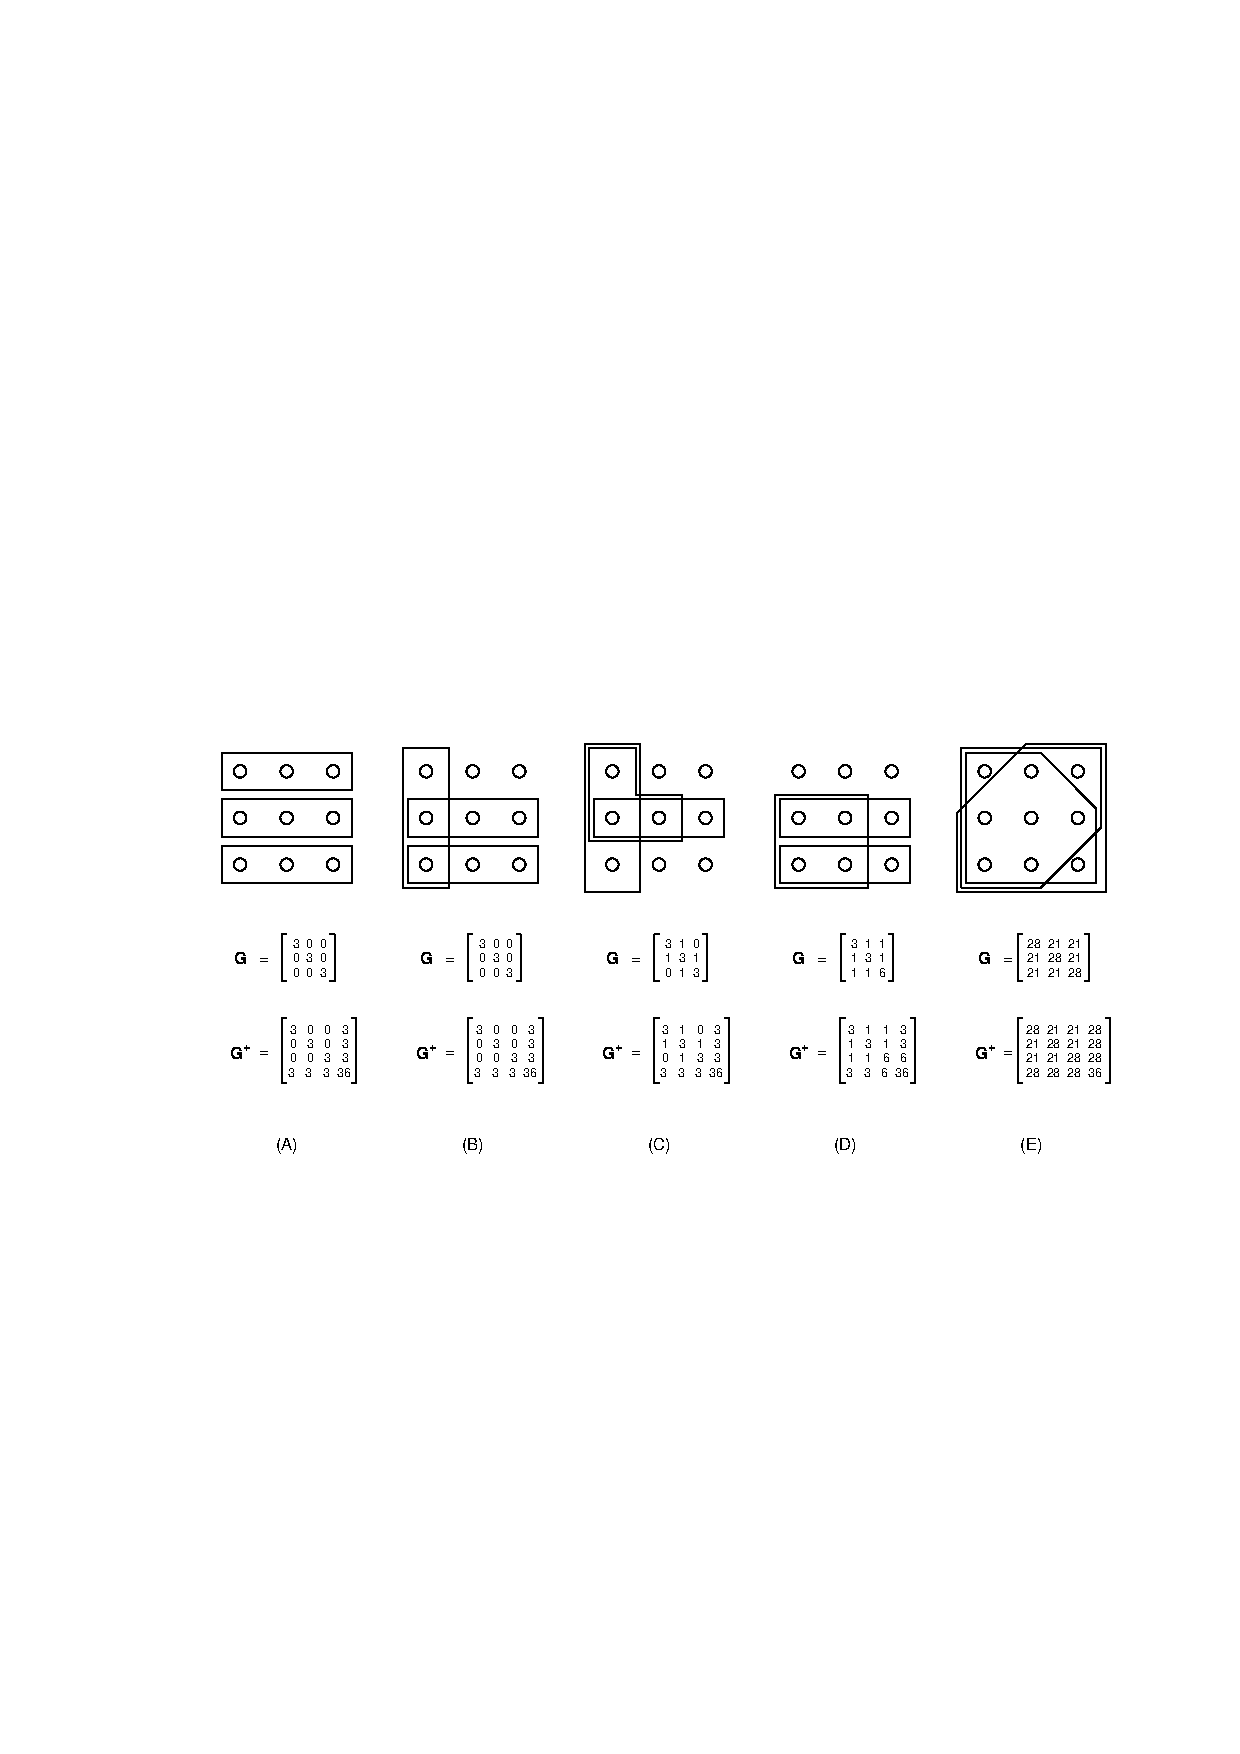
\includegraphics[width=5.99in]{features.png}
%\centereps{5.99in}{2.79in}{features.eps}
\caption{Five feature structures for a nine-stimulus domain. Feature set A has a partit\-ion\-ing structure, whereas B is an example of a non-partitioning structure that also has a diagonal complexity matrix. In set C, each cluster still encompasses three stimuli, but some overlap emerges. Feature structure D introduces a small amount of overlap at the expense of increasing the size of one cluster, whereas the features in E are large and overlap extensively. Two complexity matrices are given for each: $\mat{G}$ is the complexity matrix for the features shown, whereas $\mat{G^{+}}$ incorporates the additive constant. The $xy$-th element of a complexity matrix is obtained by counting the number of stimulus pairs common to the $x$-th and $y$-th clusters.}
\label{fig:features}
\end{figure}

The second caveat that attaches to Lee's discussion is that Hadamard's inequality applies only if the product of the main diagonal elements remains constant: that is, when the number of stimuli (and hence pairs of stimuli) in each cluster remains constant. Hadamard's inequality does not indicate what happens to the model's complexity as the number of stimuli in a cluster changes. Therefore, although Lee identifies encompassment and overlap as sources of model complexity, arguments based on Hadamard's inequality only take overlap into account. In some situations, these two factors can be varied independently: for example, a stimulus that does not belong to any cluster can be added to one of them without causing any change in the off-diagonal elements of $\mat{G}$. Similarly, the comparison between feature structures A and C in Figure~\ref{fig:features} involves manipulating the overlap between clusters without changing their size. Nevertheless, such independence is hardly the norm, and it is not immediately obvious what happens to complexity when a feature is enlarged at the expense of introducing more overlap. Consider feature structures A, D and E in Figure~\ref{fig:features}. Two of the features in A and D are identical, but the third feature in D contains four stimuli rather than three, and shares  one stimulus pair with each of the other two features. As it turns out, D is the more complex representation, with $|\mat{G}|=44$ and $|\mat{G^{+}}|=1224$ (compared to 27 and 729 for A). Feature structure E involves larger clusters and more overlap, as there are 8 stimuli in each cluster and 7 stimuli shared between all pairs of clusters, yielding $|\mat{G}|=3430$. Once the additive constant is introduced, it is no longer possible to have larger features or more overlap without including the same feature twice (which is degenerate), and $|\mat{G^{+}}|$ for this representation is 8232. In this example at least, representations with smaller clusters are simpler than those with larger clusters, even though it comes at the expense of reduced overlap.

It is also worthwhile to note that, for a fixed number of clusters the simplest representation is one consisting only of clusters containing two stimuli. The complexity matrix for this representation is the identity, and therefore has determinant 1. Since $\mat{G}$ is positive definite, its determinant must be positive, and since the elements of $\mat{G}$ are integers, no complexity matrix can ever have a determinant smaller than 1. This argument does not incorporate the additive constant, but it is heartening to note that a representation of nine stimuli using three two-stimulus clusters has $|\mat{G^{+}}|=33$, making it simpler than any of those displayed in Figure~\ref{fig:features}.

To summarize, the solid statistical foundation of Lee's \citeyear{lee01b} approximation to the Bayesian posterior lends it considerable status as a selection criterion for additive clustering models. The determinant of the complexity matrix $\mat{G}$ is a function of the size and overlap of features in the representation, but caution is required when applying Hadamard's inequality, which only takes overlap into account: in the examples presented here, representations with smaller clusters and less overlap were simpler than those with larger clusters but more overlap.

\section{Acknowledgements}
The research in this paper was financially supported by the Communications Division of the Australian Defence Science and Technology Organisation, and by an Australian Postgraduate Award. The author wishes to thank Michael Lee, Barbara Mellers, and an anonymous reviewer for helpful comments on an earlier version of this article.

\begin{thebibliography}{}

\bibitem[\protect\BCAY{Bellman}{Bellman}{1970}]{bel70}
Bellman, R.
\newblock{}\BBOP{}1970\BBCP{}.
\newblock{}\Bem{Introduction to Matrix Analysis}\ (2nd\ \BEd).
\newblock{}New York: McGraw-Hill.

\bibitem[\protect\BCAY{Kass \BBA{} Raftery}{Kass \BBA{}
  Raftery}{1995}]{kasraf95}
Kass, R.~E.\BCBT{} \BBA{} Raftery, A.~E.
\newblock{}\BBOP{}1995\BBCP{}.
\newblock{}\BBOQ{}Bayes factors.\BBCQ{}
\newblock{}\Bem{Journal of the American Statistical Association}, \Bem{90},
  773-795.

\bibitem[\protect\BCAY{Lee}{Lee}{2001}]{lee01b}
Lee, M.~D.
\newblock{}\BBOP{}2001\BBCP{}.
\newblock{}\BBOQ{}On the complexity of additive clustering models.\BBCQ{}
\newblock{}\Bem{Journal of Mathematical Psychology}, \Bem{45}, 131-148.

\bibitem[\protect\BCAY{Lee}{Lee}{2002}]{leesub3}
Lee, M.~D.
\newblock{}\BBOP{}2002\BBCP{}.
\newblock{}\BBOQ{}Generating additive clustering models with limited stochastic complexity.\BBCQ{}
\newblock{}\Bem{Journal of Classification}, \Bem{19}, 69-85.

\bibitem[\protect\BCAY{Myung, Balasubramanian\BCBL{} \BBA{} Pitt}{Myung
  \BOthers{}}{2000}]{myubalpit00}
Myung, I.~J., Balasubramanian, V.\BCBL{} \BBA{} Pitt, M.~A.
\newblock{}\BBOP{}2000\BBCP{}.
\newblock{}\BBOQ{}Counting probability distributions: Differential geometry and
  model selection.\BBCQ{}
\newblock{}\Bem{Proceedings of the National Academy of Sciences USA}, \Bem{97},
  11170-11175.

\bibitem[\protect\BCAY{Rissanen}{Rissanen}{1996}]{ris96}
Rissanen, J.
\newblock{}\BBOP{}1996\BBCP{}.
\newblock{}\BBOQ{}Fisher information and stochastic complexity.\BBCQ{}
\newblock{}\Bem{IEEE Transactions on Information Theory}, \Bem{42}(1), 40-47.

\bibitem[\protect\BCAY{Shepard \BBA{} Arabie}{Shepard \BBA{}
  Arabie}{1979}]{sheara79}
Shepard, R.~N.\BCBT{} \BBA{} Arabie, P.
\newblock{}\BBOP{}1979\BBCP{}.
\newblock{}\BBOQ{}Additive clustering representations of similarities as
  combinations of discrete overlapping properties.\BBCQ{}
\newblock{}\Bem{Psychological Review}, \Bem{86}(2), 87-123.

\end{thebibliography}

\end{document}
